\documentclass[12pt]{report}
\usepackage[utf8]{inputenc}
\usepackage{graphicx}
\usepackage{titlesec}
\usepackage{xcolor}
\usepackage{fancyhdr}
\usepackage{tikz}
\usepackage{charter}
\usepackage[table]{xcolor} 
\usepackage{float}  % Add this in the preamble
\usepackage{longtable}  
\usepackage{atbegshi} 
\usepackage{array}
\usepackage{hyperref} 
\usepackage{cellspace}
\usepackage[a4paper, left=1in, right=1in, bottom=0.8in, top=0.8in]{geometry}

% Border settings
\newlength{\mymargin}
\setlength{\mymargin}{0.8cm}
\renewcommand{\baselinestretch}{1.4} % 1.5x line height
\pagenumbering{gobble}  % Disables page numbering 
\setlength{\cellspacetoplimit}{6pt}
\setlength{\cellspacebottomlimit}{6pt}


\AtBeginShipout{%
  \AtBeginShipoutUpperLeft{%
    \begin{tikzpicture}[remember picture, overlay]
      \draw[line width=0.4pt] 
        ([xshift=\mymargin, yshift=\mymargin] current page.south west) % Bottom-left corner with margin
        rectangle 
        ([xshift=-\mymargin, yshift=-\mymargin] current page.north east); % Top-right corner with margin
    \end{tikzpicture}%
  }%
}

\begin{document}

\begin{center}
	\begin{center}\begin{minipage}
			{0.1\textwidth}

			\centering
			\hspace*{-0.7cm}
			
\includegraphics[width=2.2cm]{images/uni_logo.jpg}
		\end{minipage}%
		\hfill
		\begin{minipage}{0.7\textwidth}


			\centering
			\fontsize{12}{19}\selectfont % 14pt font with 18pt line spacing
			\textbf{People's Democratic Republic of Algeria} \\
			Ministry of Higher Education and Scientific Research \\
			\textbf{Martyr Hamma Lakhdar University of El Oued} \\

		\end{minipage}%
		\hfill
		\begin{minipage}{0.1\textwidth}

			\centering
			
\includegraphics[width=2.2cm]{images/uni_logo.jpg}
		\end{minipage}
	\end{center}
	\vspace{0.5cm}
	\fontsize{12}{20}\selectfont
	Faculty of Exact Sciences \\
	Department of Computer Science \\
	\vspace{0.5cm}
	\textbf{Graduation Project Report} \\
	License 3rd And Final Year \\
	\rule{0.85\linewidth}{0.5pt} \\[0.3cm]
	\textbf{\Large Hospital Finder Mobile App}
	\rule{0.85\linewidth}{0.5pt}  \vspace{1cm}
	\begin{flushright}
		\begin{minipage}[t]{0.8\textwidth} % Total width of both columns
			\begin{minipage}[t]{0.48\textwidth}
				\hspace*{-1.7cm}
				\textbf{Prepared by:} \\[-7.7ex]
				\begin{itemize} \setlength\itemsep{0em}
					\setlength\itemsep{-0.8em}
					\setlength\labelsep{2cm}
					\setlength\labelwidth{0.5cm}
					\item \hspace*{-1.9cm} Gouder Hicham
					\item \hspace*{-1.9cm} Guedda Alla
					\item \hspace*{-1.9cm} Ayoub Zekri
				\end{itemize}

			\end{minipage}%
			\hfill
			\begin{minipage}[t]{0.48\textwidth}
				\hspace*{0.5cm}
				\textbf{Supervised by:} \\[-7.7ex]
				\begin{itemize} \setlength\itemsep{0em}
					\setlength\itemsep{-0.8em}
					\setlength\labelsep{-0.2cm}
					\setlength\labelwidth{0.5cm}
					\item \hspace*{0.3cm} Sasci Mdileh
				\end{itemize}
			\end{minipage}
		\end{minipage}
	\end{flushright}
	\vspace{5cm}
	\Large Academic Year: 2024/2025 \\
	\vfill
\end{center}
\tableofcontents
\newpage
\begin{center}
	\textbf{Abstract} \\
	\vspace*{0.3cm}
\end{center}
\noindent In many regions, private medical clinics and hospitals are widespread, making it difficult for residents and visitors to locate suitable healthcare facilities quickly.

\noindent Patients often struggle to find nearby hospitals, determine the best routes, or identify available medical services, especially in emergencies. This challenge is particularly significant for individuals unfamiliar with the area or those seeking specialized medical care.

\noindent To address this issue, we propose the development of a mobile application that enables users to geolocate hospitals and medical clinics efficiently.
\vspace*{0.5cm}

\noindent The application integrates mapping services to provide accurate locations and essential details about healthcare institutions. Additionally, it allows users to contact clinics directly via phone for inquiries and appointments. \vspace*{0.5cm}

\noindent By offering a user-friendly interface and real-time location-based services, this application aims to enhance accessibility to healthcare facilities, improve navigation for patients, and support better healthcare decision-making.  \vspace*{0.5cm}


\noindent \vspace*{0.5cm}\textbf{Keywords:} Mobile Application, Android, Geolocation, Google Maps.
\newpage
\begin{center}
	\textbf{Acknowledgment} \\
	\vspace*{0.3cm}
\end{center}

\noindent I would like to express my gratitude to everyone who contributed to the completion of this project. Their support and guidance played a significant role in its successful development.  \vspace*{0.5cm}

\noindent First, I extend my sincere appreciation to my supervisor, \textbf{Sassi Mdileh}, for his valuable guidance, feedback, and support throughout this work. Their expertise and constructive advice have been essential in refining the project and addressing challenges effectively.

\noindent I also thank the faculty members of the \textbf{Faculty of Exact Sciences} for their insights and recommendations, which have helped improve the quality of this work.  \vspace*{0.5cm}

\noindent Furthermore, I appreciate the efforts of my colleagues, for their collaboration and commitment. Their contributions were crucial in different stages of the project, and their teamwork helped ensure its completion.  \vspace*{0.5cm}

\noindent I would also like to acknowledge the administrative and technical staff at the faculty for providing necessary resources and assistance throughout the process.  \vspace*{0.5cm}

\noindent Finally, I am grateful to my family for their continuous support and encouragement. Their patience and understanding allowed me to stay focused on this project.

\newpage

\addcontentsline{toc}{chapter}{General Introduction}










% ========================= ======================== = = = = 

\section*{\textbf{1. Introduction}}
\rule{\linewidth}{1pt}  % Full-width horizontal line (adjust thickness if needed)


\addcontentsline{toc}{section}{1. Introduction}

\subsection*{\textbf{1.1 Project Presentation}}
\addcontentsline{toc}{subsection}{1.1 Project Presentation}

In today's fast-paced world, \textbf{access to healthcare services} is a fundamental need. However, finding the right hospital at the right time remains a \textbf{challenge} for many individuals. Whether it is for \textbf{emergency cases, routine check-ups, or specialized consultations}, people often struggle to locate nearby healthcare facilities that match their needs.

\noindent Traditional methods of searching for hospitals—such as \textbf{word-of-mouth recommendations or general internet searches}—are often \textbf{inefficient, time-consuming, and unreliable}. They rarely provide crucial details such as:
\begin{itemize}
	\item \textbf{Hospital specialties}
	\item \textbf{Available doctors and their expertise}
	\item \textbf{Operating hours and emergency services}
	\item \textbf{Real-time availability of services}
\end{itemize}

\noindent To address these challenges, we propose the development of a \textbf{Hospital Finder Mobile Application}. This app aims to help users \textbf{quickly and efficiently} locate nearby hospitals based on various criteria such as \textbf{location, specialty, available services, and real-time availability}. By integrating \textbf{modern technologies like geolocation, search filtering, and live data updates}, our system provides an \textbf{intelligent, user-friendly, and accessible solution} for patients and healthcare professionals.

\subsection*{\textbf{1.2 Application Objectives}}
\addcontentsline{toc}{subsection}{1.2 Application Objectives}

The primary goal of this application is to \textbf{simplify the process of finding hospitals and healthcare facilities} while ensuring users receive the most relevant and \textbf{real-time} information. Specifically, the application aims to:

\begin{itemize}
	\item \textbf{Improve Accessibility to Healthcare Services:} Provide an intuitive platform for users to locate hospitals, clinics, and medical specialists.
	\item \textbf{Enhance Patient Decision-Making:} Offer users hospital \textbf{ratings, available doctors, specialization areas, and real-time service availability}.
	\item \textbf{Reduce Search Time:} Optimize search and filtering functionalities to help users find the best hospital quickly.
	\item \textbf{Integrate Geolocation Services:} Enable real-time location tracking to suggest \textbf{the closest and most relevant medical facilities}.
	\item \textbf{Facilitate Patient-Hospital Communication:} Provide direct contact options such as \textbf{phone calls, appointment booking, and navigation assistance}.
\end{itemize}

\noindent By implementing these objectives, the \textbf{Hospital Finder Mobile Application} seeks to \textbf{enhance healthcare accessibility} and \textbf{reduce the time required to locate medical facilities}.

\subsection*{\textbf{1.3 Methodology and Adopted Formalisms}}
\addcontentsline{toc}{subsection}{1.3 Methodology and Adopted Formalisms}

To develop the \textbf{Hospital Finder Mobile Application}, we followed a structured approach, combining:
\begin{itemize}
	\item \textbf{Theoretical Study}
	\item \textbf{Technical Analysis}
	\item \textbf{Practical Implementation}
\end{itemize}

Our methodology consists of the following key steps:

\begin{enumerate}
	\item \textbf{Preliminary Study and Research}
	      \begin{itemize}
		      \item Analyze existing hospital-finder applications and their \textbf{limitations}.
		      \item Identify key \textbf{user needs and expectations} through research and surveys.
	      \end{itemize}

	\item \textbf{Requirement Specification and System Analysis}
	      \begin{itemize}
		      \item Define the \textbf{functional and non-functional requirements} of the system.
		      \item Develop \textbf{use case diagrams, system architecture, and database design} to ensure a structured implementation.
	      \end{itemize}

	\item \textbf{Design and Development}
	      \begin{itemize}
		      \item Implement a \textbf{cross-platform mobile application}.
		      \item Utilize \textbf{Flutter for the front-end} to ensure compatibility with both Android and iOS.
		      \item Store and manage data using \textbf{Firebase and a structured database modify later}.
	      \end{itemize}

	\item \textbf{Testing and Validation}
	      \begin{itemize}
		      \item Conduct rigorous \textbf{functionality, performance, and security} testing.
		      \item Gather \textbf{user feedback} and refine the app based on real-world usage.
	      \end{itemize}

	\item \textbf{Deployment and Future Enhancements}
	      \begin{itemize}
		      \item Deploy the application for public use, ensuring \textbf{a smooth user experience}.
		      \item Plan for \textbf{future updates}, including:
		            \begin{itemize}
			            \item \textbf{AI-based hospital recommendations modify later}
			            \item \textbf{Telemedicine features}
			            \item \textbf{Integration with electronic health records (EHR)}
		            \end{itemize}
	      \end{itemize}
\end{enumerate}









\newpage

\chapter{\textbf{Theoretical Study and Technical Choices}}
\rule{\linewidth}{1.5pt}


\section{\textbf{Introduction}}

In today's digital age, access to precise and reliable healthcare information is essential. Many existing applications provide hospital location services, but they often lack \textbf{detailed and accurate clinic information}.
This chapter explores the theoretical aspects of our \textbf{Hospital Finder Mobile Application}, analyzes existing solutions, and presents our improved approach.

\section{\textbf{Preliminary Study}}
\vspace{-0.5cm}
\rule{7.5cm}{1.5pt}
\vspace{-0.5cm}
\subsection{\textbf{Study of Existing Solutions: Geolocation, Search on Google Maps, …}}

Several solutions exist for finding hospitals and clinics, but they have \textbf{significant limitations}:

\begin{itemize}
	\item \textbf{Google Maps:}
	      Google Maps is the most widely used mapping service, offering general hospital searches. However, it \textbf{lacks precise information on clinics}, including doctors' availability, specialties, and operating hours.
	\item \textbf{Hospital Finder by Darshan University:}
	      This global application \textbf{only fetches hospital data from the Google Maps API} without allowing clinics to \textbf{add or modify their information}. Additionally, its \textbf{user interface is outdated}, making navigation difficult.
	\item \textbf{Local Availability:}
	      Currently, \textbf{no local application} provides a \textbf{dedicated hospital and clinic management system} that allows clinics to \textbf{register themselves, update details, and display real-time doctor availability}.
\end{itemize}

\subsection{\textbf{Critique of Existing Solutions and Proposed Solution}}

\textbf{Limitations of Existing Solutions:}
\begin{itemize}
	\item No \textbf{custom clinic registration} or modifications
	\item Outdated UI and poor \textbf{user experience}
	\item No \textbf{detailed doctor profiles and schedules}
	\item Google Maps data is \textbf{too general} and lacks \textbf{localized clinic information}
\end{itemize}

\noindent \textbf{Proposed Solution:}
To overcome these limitations, our \textbf{Hospital Finder Mobile Application} introduces:
\begin{itemize}
	\item \textbf{Enhanced Geolocation} → Provides \textbf{precise clinic locations} added by clinic administrators themselves.
	\item \textbf{Clinic Registration \& Management} → Clinics can \textbf{create, modify, and update their information}.
	\item \textbf{Detailed Doctor Profiles} → Displays \textbf{doctor specialties, working hours, availability, and schedules}.
	\item \textbf{Nearby Hospital \& Clinic Recommendations} → Suggests hospitals and clinics \textbf{based on real-time location}.
	\item \textbf{Modern UI \& Better User Experience} → A \textbf{new, intuitive, and visually appealing interface}.
\end{itemize}

\section{\textbf{Conclusion}}

The existing hospital location solutions fail to provide \textbf{detailed, precise, and user-friendly} hospital and clinic information. Our \textbf{Hospital Finder Mobile Application} bridges this gap by offering:
\begin{itemize}
	\item A \textbf{better geolocation system} for \textbf{more accurate clinic placement}.
	\item The ability for \textbf{clinics to register and update their details}.
	\item \textbf{Comprehensive doctor profiles}, making hospital visits more efficient.
	\item \textbf{A modern UI} with an intuitive design for easy navigation.
\end{itemize}

\noindent This enhanced system will significantly improve \textbf{healthcare accessibility} and provide a \textbf{better user experience} compared to existing solutions.











\newpage

\chapter{\textbf{Analysis and Specification of Requirements}}
\rule{\linewidth}{1.5pt}  % Full-width underline  

\section{\textbf{Introduction}}

\noindent To develop an efficient and user-friendly \textbf{Hospital Finder Mobile Application}, it is crucial to analyze the key actors involved, their roles, and the functional and non-functional requirements. This chapter presents an in-depth study of the application’s requirements and specifications.

\section{\textbf{Global Analysis of the Application}}

\noindent This section defines the main actors interacting with the system, along with their respective tasks and permissions. The application has four primary actors:
\begin{itemize}
	\item \textbf{User} – Searches for hospitals and doctors.
	\item \textbf{Clinic} – Registers doctors and manages clinic information.
	\item \textbf{Doctor} – Manages schedules and appointments.
	\item \textbf{Admin} – Approves new clinics and ensures system integrity.
\end{itemize}

\subsection{\textbf{User Definition}}
\noindent A \textbf{user} is a person who enters the application to access services such as searching for nearby clinics and doctors. Users do not need special registration and can quickly access relevant information.

\subsubsection{\textbf{Main Tasks of a User}}
\begin{itemize}
	\item \textbf{Find Nearby Clinics:} View their locations on the map.
	\item \textbf{Find Available Doctors:} Check their specialties and schedules.
	\item \textbf{View Clinic Schedules:} Check the availability of clinics and doctors.
	\item \textbf{Contact Clinics:} Get phone numbers for appointments and inquiries.
\end{itemize}

\vspace{0.5cm}

\subsection{\textbf{Clinic Definition}}

\noindent A \textbf{clinic} is an entity that registers in the application to add doctors and manage their data. Registration is not automatic; an admin must approve the clinic before it becomes active.

\subsubsection{\textbf{Main Tasks of a Clinic}}
\begin{itemize}
	\item \textbf{Enter Clinic Information:} Name, address, phone number, specialties.
	\item \textbf{Wait for Admin Approval:} The clinic remains inactive until approval.
	\item \textbf{Manage Doctors:} Once approved, the clinic can:
	      \begin{itemize}
		      \item Add doctors to the system.
		      \item Provide login credentials (email and password) to doctors.
	      \end{itemize}
\end{itemize}

\vspace{0.5cm}
\subsection{\textbf{Doctor Definition}}
\noindent A \textbf{doctor} is a user who receives login credentials from the clinic they work at. Doctors cannot register independently but are added by their respective clinics.

\subsubsection{\textbf{Doctor Tasks}}
\begin{itemize}
	\item \textbf{Login:} Use the email and password provided by the clinic.
	\item \textbf{Manage Schedule:} Set availability and update consultation hours.
	\item \textbf{Receive Appointments:} Accept patient calls and schedule visits.
\end{itemize}

\vspace{0.5cm}


\subsection{\textbf{Admin Definition}}

\noindent The \textbf{admin} is responsible for approving or rejecting newly registered clinics. They have a separate admin application to manage the system efficiently.

\subsubsection{\textbf{Admin Tasks}}
\begin{itemize}
	\item \textbf{Review Clinic Registration Requests:} Check clinic information for validity.
	\item \textbf{Approve or Reject Clinics:} Grant or deny access based on verification.
	\item \textbf{Ensure System Integrity:} Monitor and manage the overall platform.
\end{itemize}


















\subsection{App Users Roles Table}
\noindent The application consists of multiple user roles, each with distinct responsibilities and functionalities. Understanding these roles is essential for ensuring smooth operation and proper management within the system. Below is a breakdown of the key roles and their main tasks:

% Longtable for splitting across pages
\renewcommand{\arraystretch}{1.3} % Adjust row spacing

\begin{longtable}{|p{3cm}|p{6cm}|p{6cm}|}
	
	\hline
	\rowcolor[HTML]{C0C0C0}
	\hspace*{1cm}\textbf{Role}                                                                               & \hspace*{1.9cm} \textbf{Definition}                                                                 & \hspace*{1.9cm}\textbf{Main Tasks} \\
	\hline
	\endfirsthead

	\hline
	\rowcolor[HTML]{C0C0C0}
	\hspace*{1cm}\textbf{Role}                                                                                              & \hspace*{1.9cm} \textbf{Definition}                                                                 & \hspace*{1.9cm}\textbf{Main Tasks} \\
	\hline
	\endhead

	\hspace*{0.1cm}\textbf{User (Patient)}                                                                                    & A person accessing the app to find clinics and doctors without registration.        &
	• Search for nearby clinics and doctors.\newline
	• View doctor specialties and clinic details.\newline
	• Check clinic and doctor schedules.\newline
	• Contact clinics for appointments.                                                                                                                                                                                    \\
	\hline

	\hspace*{0.9cm}\textbf{Clinic}                                                                                            &
	An entity that registers on the app to manage doctors and provide services. Approval by admin is required. &
	• Register and provide clinic details.\newline
	• Wait for admin approval.\newline
	• Add and manage doctors.\newline
	• Provide login credentials to doctors.                                                                                                                                                                                \\
	\hline


	\hspace*{0.85cm}\textbf{Doctor}                                                                                            & A medical professional registered under a clinic who cannot independently sign up.  &
	• Log in with clinic-provided credentials.\newline
	• Manage and update their schedule.\newline
	• Receive and manage patient appointments.                                                                                                                                                                             \\
	\hline

	\hspace*{0.85cm}\textbf{Admin}                                                                                             & The system manager responsible for approving clinics and ensuring smooth operation. &
	• Review and approve/reject clinic registrations.\newline
	• Monitor system performance and security.\newline
	• Ensure proper functionality of the platform.                                                                                                                                                                         \\
	\hline


\end{longtable}




























\subsection{Conclusion}
This document has provided an overview of the system, focusing on the roles and responsibilities of users. The Hospital Finder Mobile App ensures smooth interaction between patients, clinics, and administrators.
\vspace{0.5cm}
\section{\textbf{Functional Requirements Specification}}

\noindent The functional requirements define the expected behavior of the application. These include:

\begin{itemize}
	\item \textbf{User Authentication:} Clinics, doctors, and admins must log in securely.
	\item \textbf{Geolocation Services:} Users can find nearby clinics and doctors with precise locations.
	\item \textbf{Clinic and Doctor Management:} Clinics can add doctors, and doctors can update their availability.
	\item \textbf{Appointment Booking:} Users can call clinics and book appointments.
	\item \textbf{Admin Panel:} The admin can approve or reject clinic registrations.
\end{itemize}

\section{\textbf{Non-Functional Requirements Specification}}

\noindent The non-functional requirements define the application's quality attributes, such as performance, security, and usability.

\begin{itemize}
	\item \textbf{Performance:} The application should provide quick search results with minimal load time.
	\item \textbf{Security:} User data must be encrypted, and authentication should be secure.
	\item \textbf{Scalability:} The system should handle a growing number of users and clinics efficiently.
	\item \textbf{User-Friendly Interface:} The UI should be intuitive and responsive across all devices.
\end{itemize}


\section{\textbf{Use Case Diagrams}}
\rule{0.45\linewidth}{0.7pt}
\subsection{\textbf{Definition of Use Case Diagrams}}


\noindent A \textbf{Use Case Diagram} is a visual representation that describes the interactions between users (actors) and the system. It outlines the different functionalities provided by the application and the roles of each user in relation to those functionalities.

\noindent These diagrams are part of \textbf{Unified Modeling Language (UML)} and help in understanding how users engage with the application. The primary components of a use case diagram include:

\begin{itemize}
	\item \textbf{Actors:} Represent users or external systems interacting with the application.
	\item \textbf{Use Cases:} Define specific actions that users can perform in the system.
	\item \textbf{Associations:} Indicate the relationship between actors and their use cases.
	\item \textbf{System Boundary:} Defines the scope of the application by enclosing all the use cases.
\end{itemize}

\noindent The goal of these diagrams is to **provide a clear, high-level understanding** of how different actors interact with the system’s functionalities, making it easier for developers, stakeholders, and designers to visualize and refine the system requirements.

\subsection{\textbf{Use Case Diagrams for the Application}}

\noindent Below are the key \textbf{Use Case Diagrams} representing interactions for different roles in the \textbf{Hospital Finder Mobile Application}.

\subsubsection{\textbf{Doctor Interactions}}
The following diagram illustrates how a doctor interacts with the application. Doctors have limited access and can only perform actions related to their schedules and patient appointments.

\vspace{0.5cm}
\noindent \textbf{Use Case Diagram: Doctor Using the App}
\begin{center}
	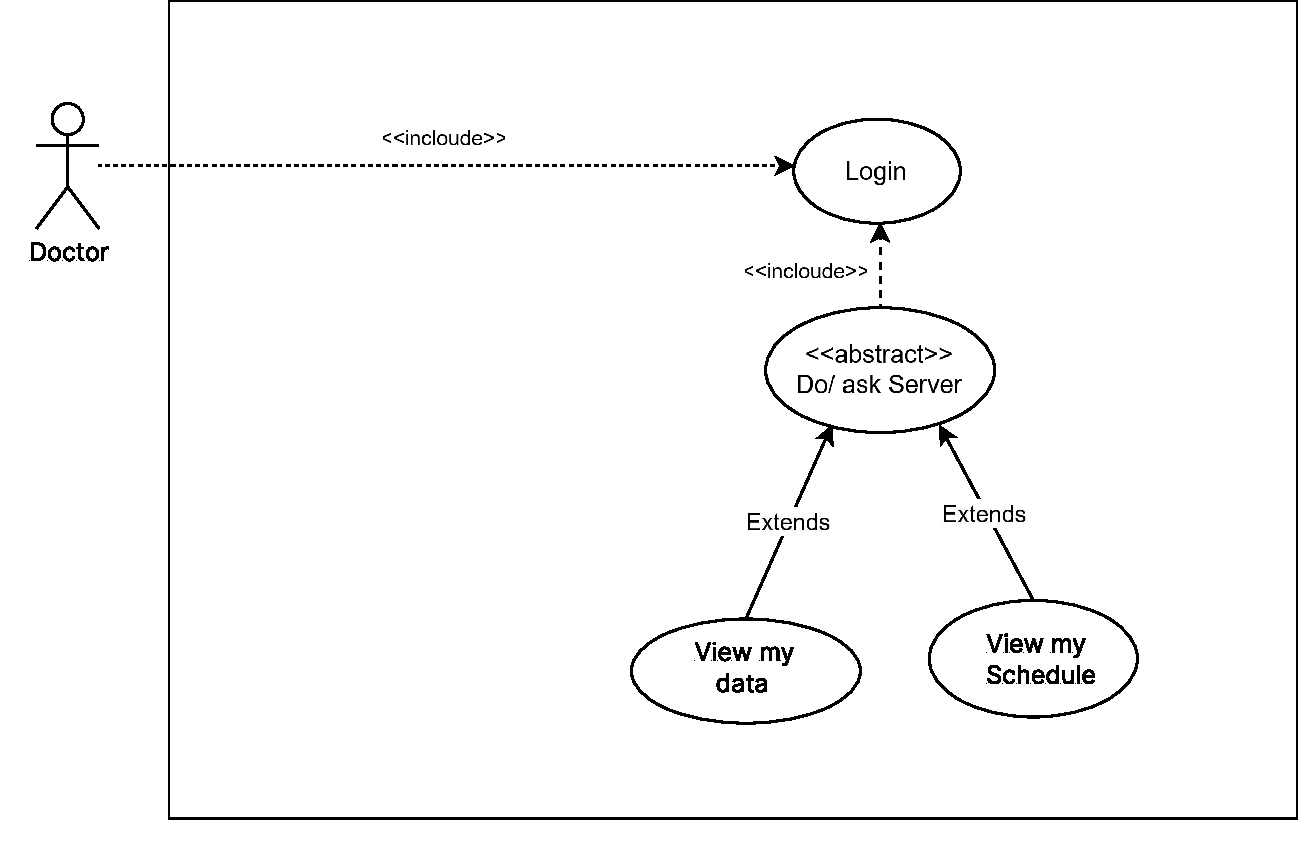
\includegraphics[width=\textwidth]{images/doctorCAS.pdf} % Replace "diagram.pdf" with your actual filename
\end{center}

\subsubsection{\textbf{User Interactions (Patients)}}
Users or patients use the application to find nearby clinics and doctors, check their schedules, and obtain contact details for appointments.

\vspace{0.5cm}
\noindent \textbf{Use Case Diagram: Patient or User Using the App}
\begin{center}
	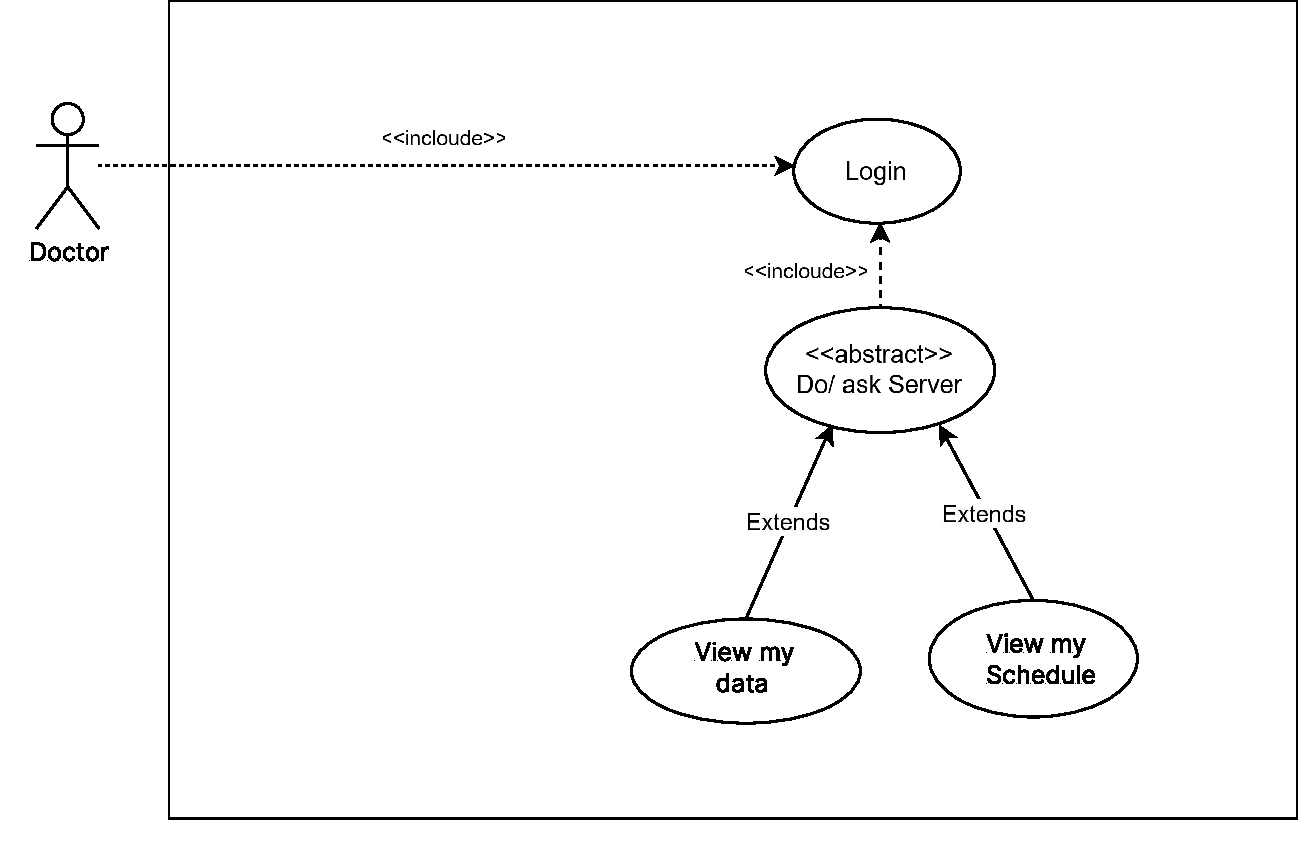
\includegraphics[width=\textwidth]{images/doctorCAS.pdf} % Replace "diagram.pdf" with your actual filename
\end{center}

\subsubsection{\textbf{Clinic Interactions}}
Clinics are responsible for registering in the application, adding doctors, and managing their clinic details. They must be approved by an admin before becoming active.

\vspace{0.5cm}
\noindent \textbf{Use Case Diagram: Clinic Using the App}
\begin{center}
	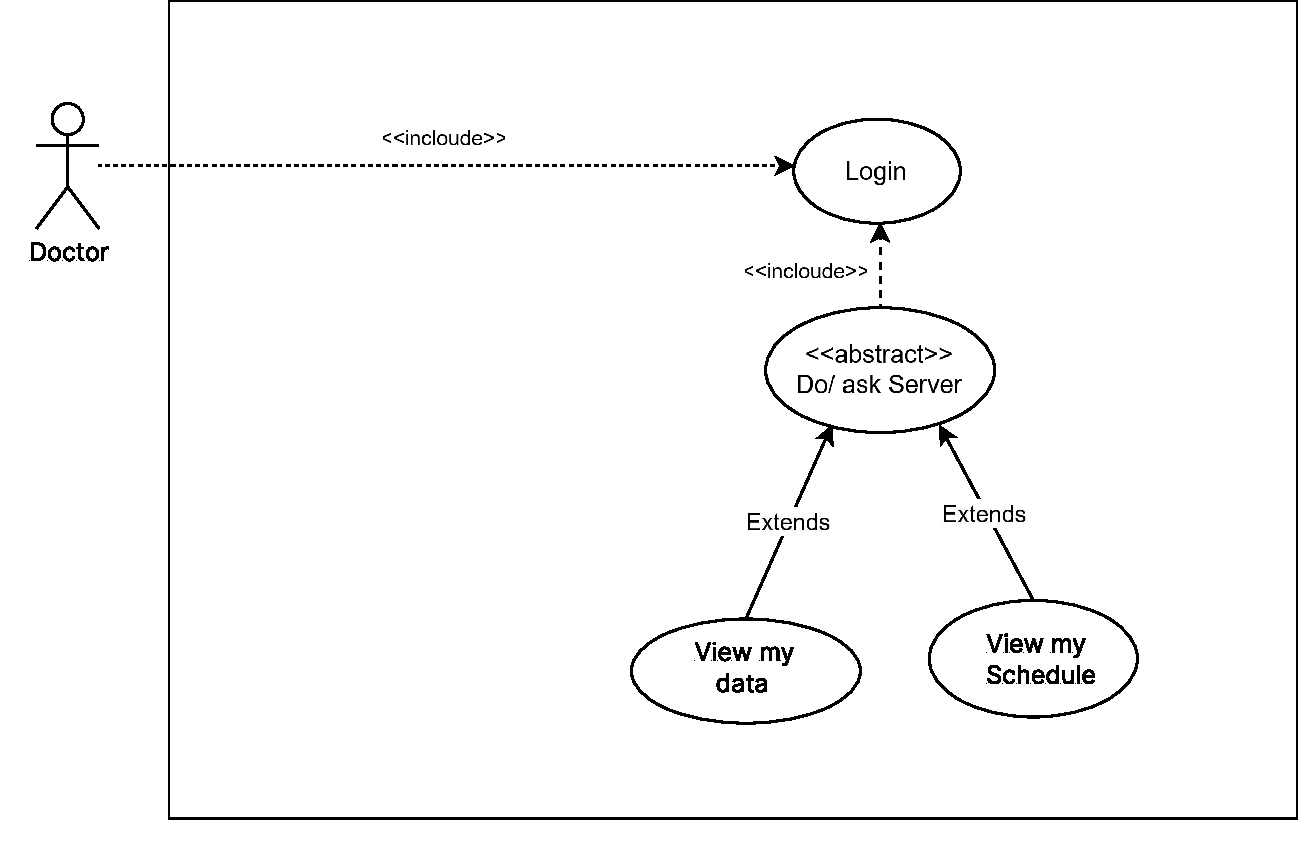
\includegraphics[width=\textwidth]{images/doctorCAS.pdf} % Replace "diagram.pdf" with your actual filename
\end{center}

\subsubsection{\textbf{Admin Interactions}}
Admins ensure the integrity of the platform by reviewing clinic registration requests and either accepting or rejecting them. They also monitor system performance and maintain security.

\vspace{0.5cm}
\noindent \textbf{Use Case Diagram: Admin Using the App}
\begin{center}
	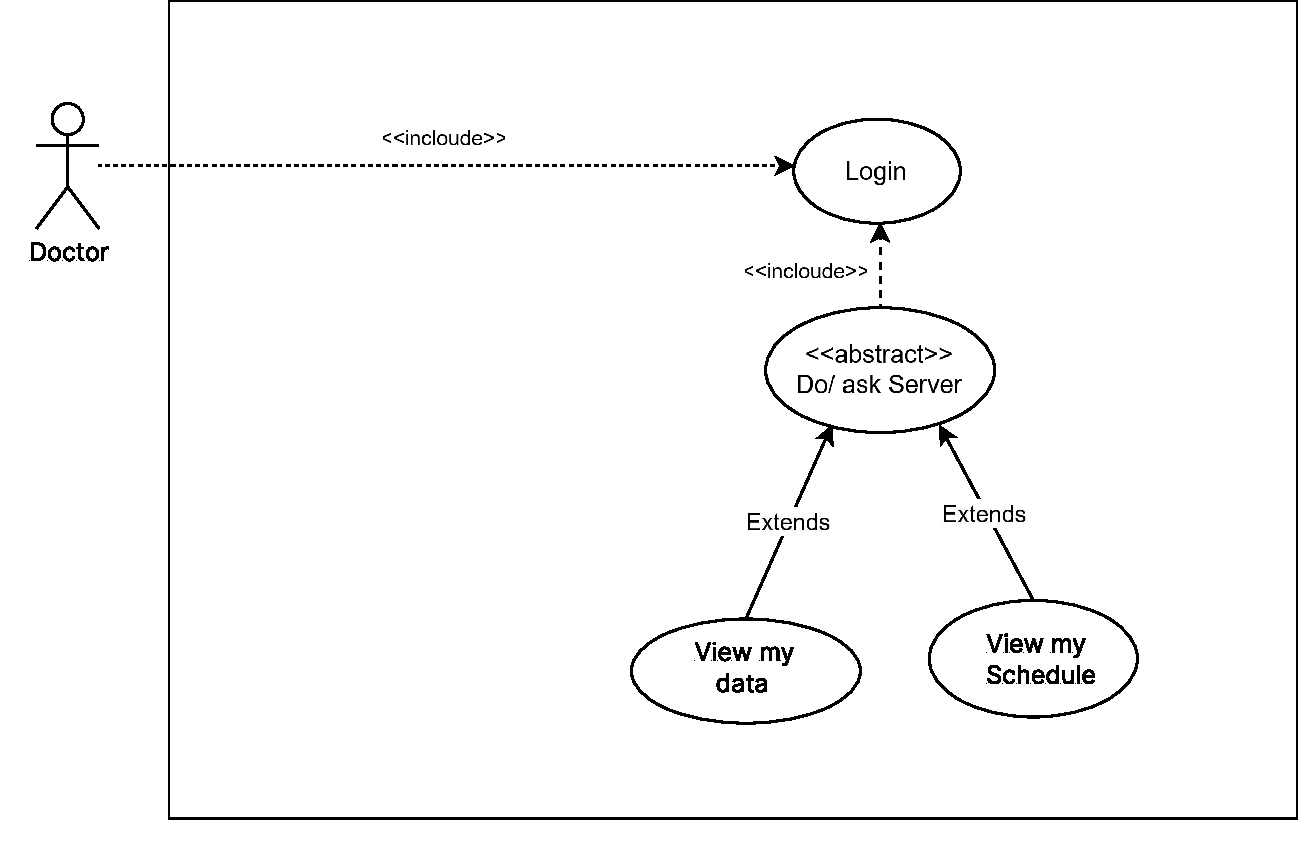
\includegraphics[width=\textwidth]{images/doctorCAS.pdf} % Replace "diagram.pdf" with your actual filename
\end{center}

\section{\textbf{Conclusion}}
\noindent This section has provided a detailed overview of \textbf{Use Case Diagrams} and their role in defining user interactions within the \textbf{Hospital Finder Mobile Application}. By mapping out different functionalities for doctors, users, clinics, and admins, these diagrams offer a structured approach to understanding the system's behavior.

\noindent The next steps involve designing the database structure and implementing the system based on these well-defined interactions.




\end{document}